\chapter{SOLID}

\section{Analyse Single-Responsibility-Principle (SRP)}

\subsubsection{Positiv-Beispiel:}

\begin{wrapfigure}{r}{0.40\textwidth}
	\centering
	\vspace{-30pt} % Manchmal möchte man den oberen Abstand selbst anpassen
	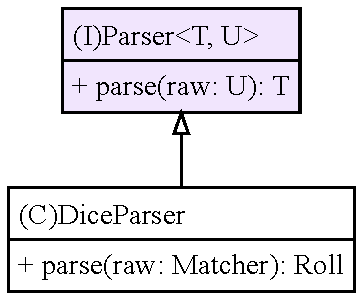
\includegraphics[width=0.30\textwidth]{Bilder/DiceParser_structure.pdf}
	\vspace{-10pt}
	% Das folgende ist ein Trick, um "Abbilgung x.y" in eine
	% eigene Zeile zu packen. Der Text zwischen [ und ] steht
	% im Abbildungsverzeichnis. Der Text darunter wird
	% tatsächlich angezeigt.
	\caption[UML-Diagramm von ase.plugin.cli.parsers.DiceParser.]{\unskip}
	UML-Diagramm von \textit{ase.plugin.cli.parsers.DiceParser}.
	\label{fig:srp-DiceParser}
\end{wrapfigure}

\autoref{fig:srp-DiceParser} zeigt das UML-Klassendiagramm des \textit{DiceParser}, welcher in der Plugin-Schicht
unter \texttt{plugin.cli.parsers} zu finden ist und das Positiv-Beispiel darstellt. 
Dieser implementiert das \textit{Parser}-Interface aus 
\texttt{plugin.cli}. Die einzige Aufgabe des DiceParsers ist es die Usereingabe zum Erstellen eines Würfelwurfs
aus Text zu parsen und das entsprechende Objekt zu kreieren. Hierzu wird der \textit{Regex}-Matcher, der 
bereits den Syntax überprüft hat an die \textit{parse}-Methode übergeben und daraus die Arugmente extrahiert, 
um den \textit{Roll} zu erstellen.

\subsubsection{Negativ-Beispiel:}

\autoref{fig:srp-RollHandler} zeig das UML-Klassendiagramm des \textit{RollHandler}, welcher in der Applikations-Schicht
die Würfelwürfe für die Rettungen (\textit{Endeavor}) \underline{und} Kämpfe (\textit{Encounter}) bearbeitet. 
Hierbei entscheidet die öffentliche \textit{handle}-Methode, ob es sich um einen Encounter oder ein Endeavor handelt
(dies ist allerdings eigentlich schon bei Aufruf dieser bekannt)
und führt die entsprechende private Methode aus. Die Klasse hat also zwei Aufgaben (Responsibilities). \\
Um dies zu lösen kann einfach die Klasse \textit{RollHandler} in zwei Klassen aufgeteilt werden - 
den \textit{EncounterHandler} und \textit{EndeavorHandler} - die nun jeweils nur noch genau eine Aufgabe haben 
und somit das SRP einhalten, wie \autoref{fig:srp-RollHandler-fixed} zeigt. 

\begin{figure}[H]
	\centering
	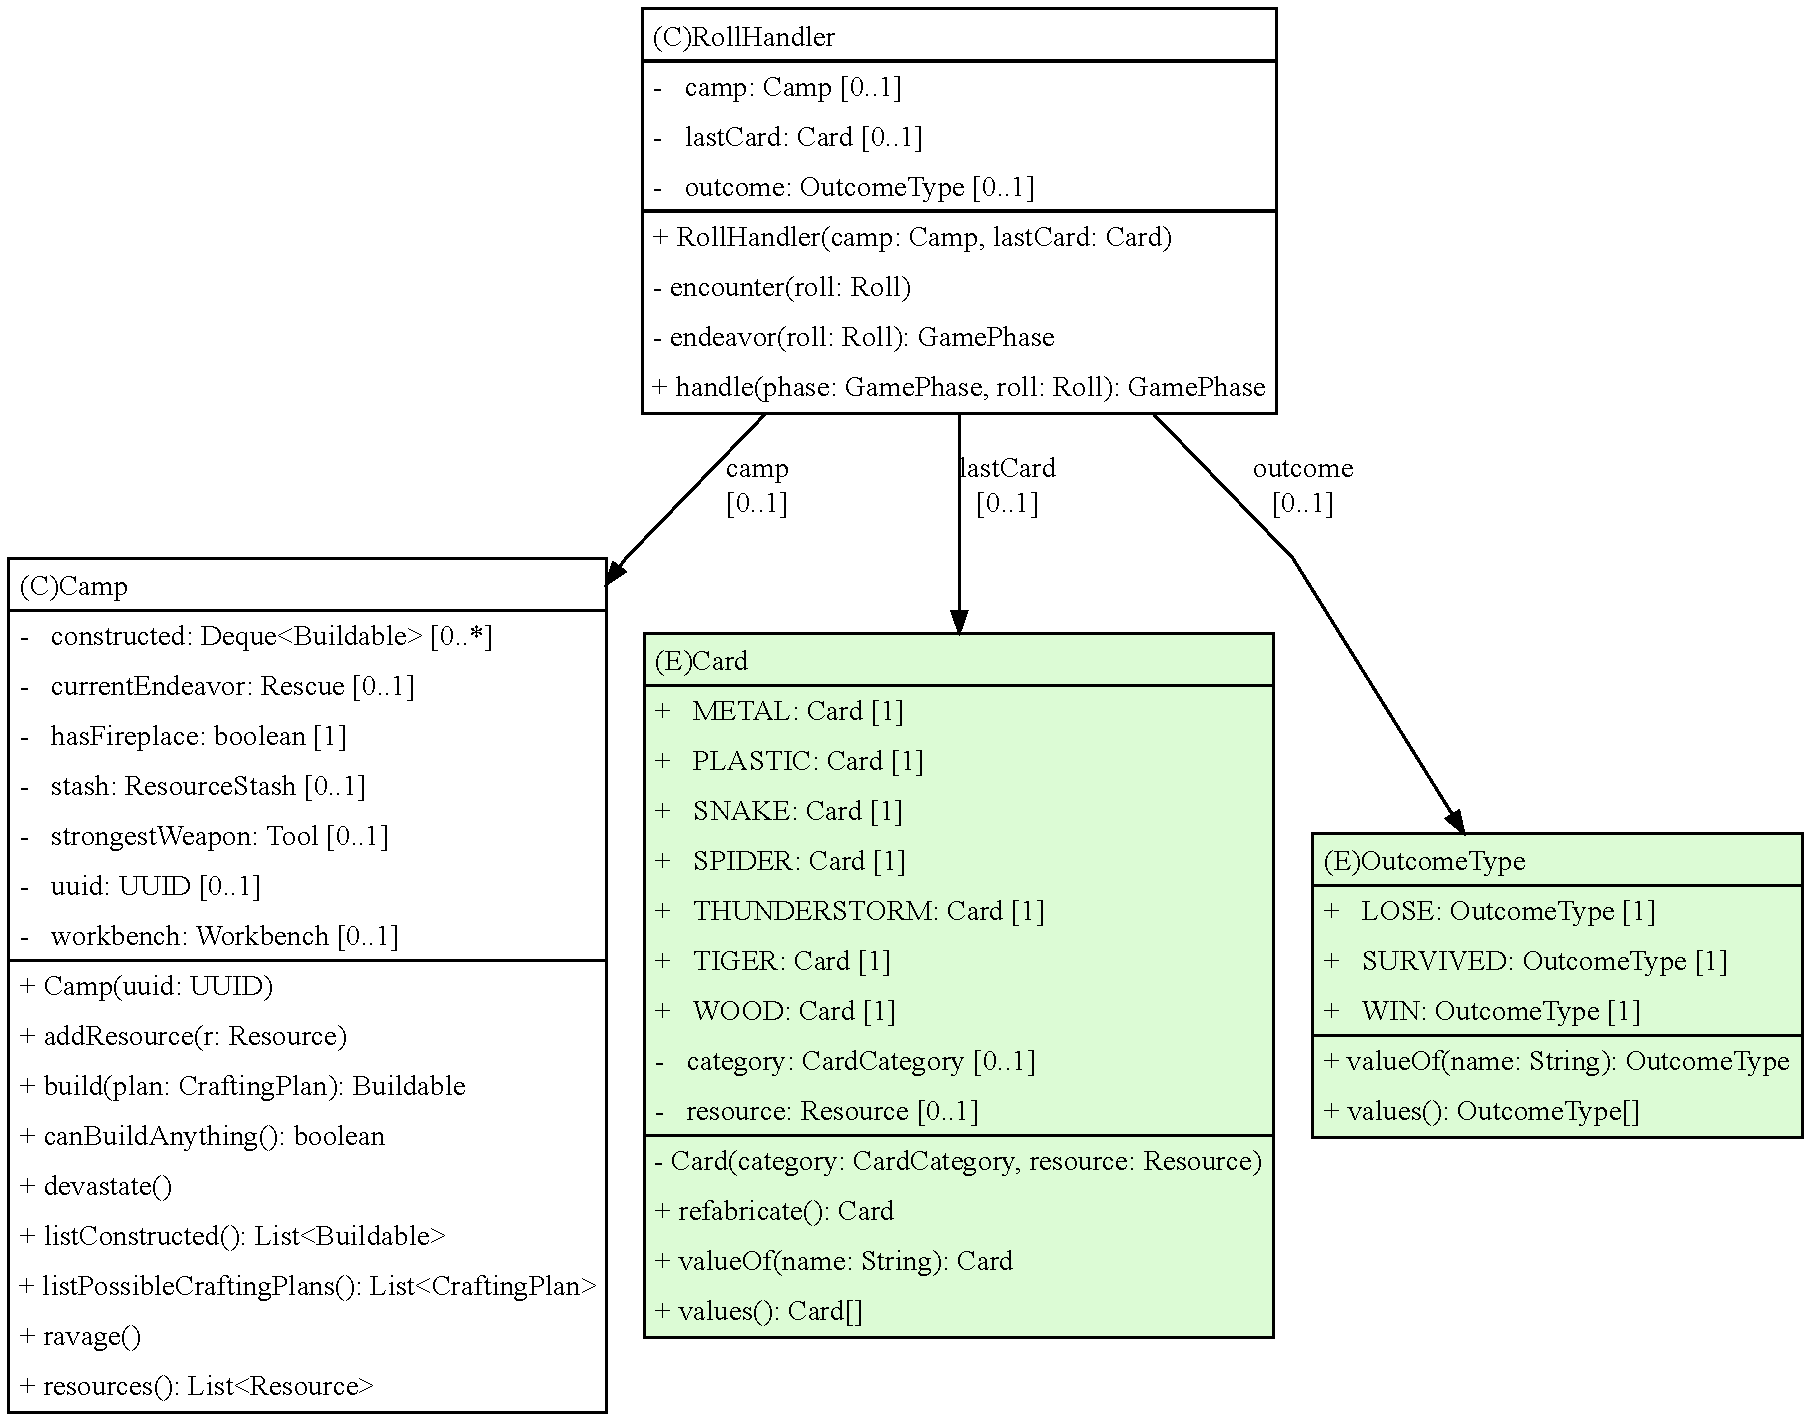
\includegraphics[width=1.\textwidth]{Bilder/RollHandler_structure.pdf} 
	\caption{UML-Diagramm von \textit{application.RollHandler}.}
	\label{fig:srp-RollHandler}
\end{figure} 

\begin{figure}[H]
	\centering
	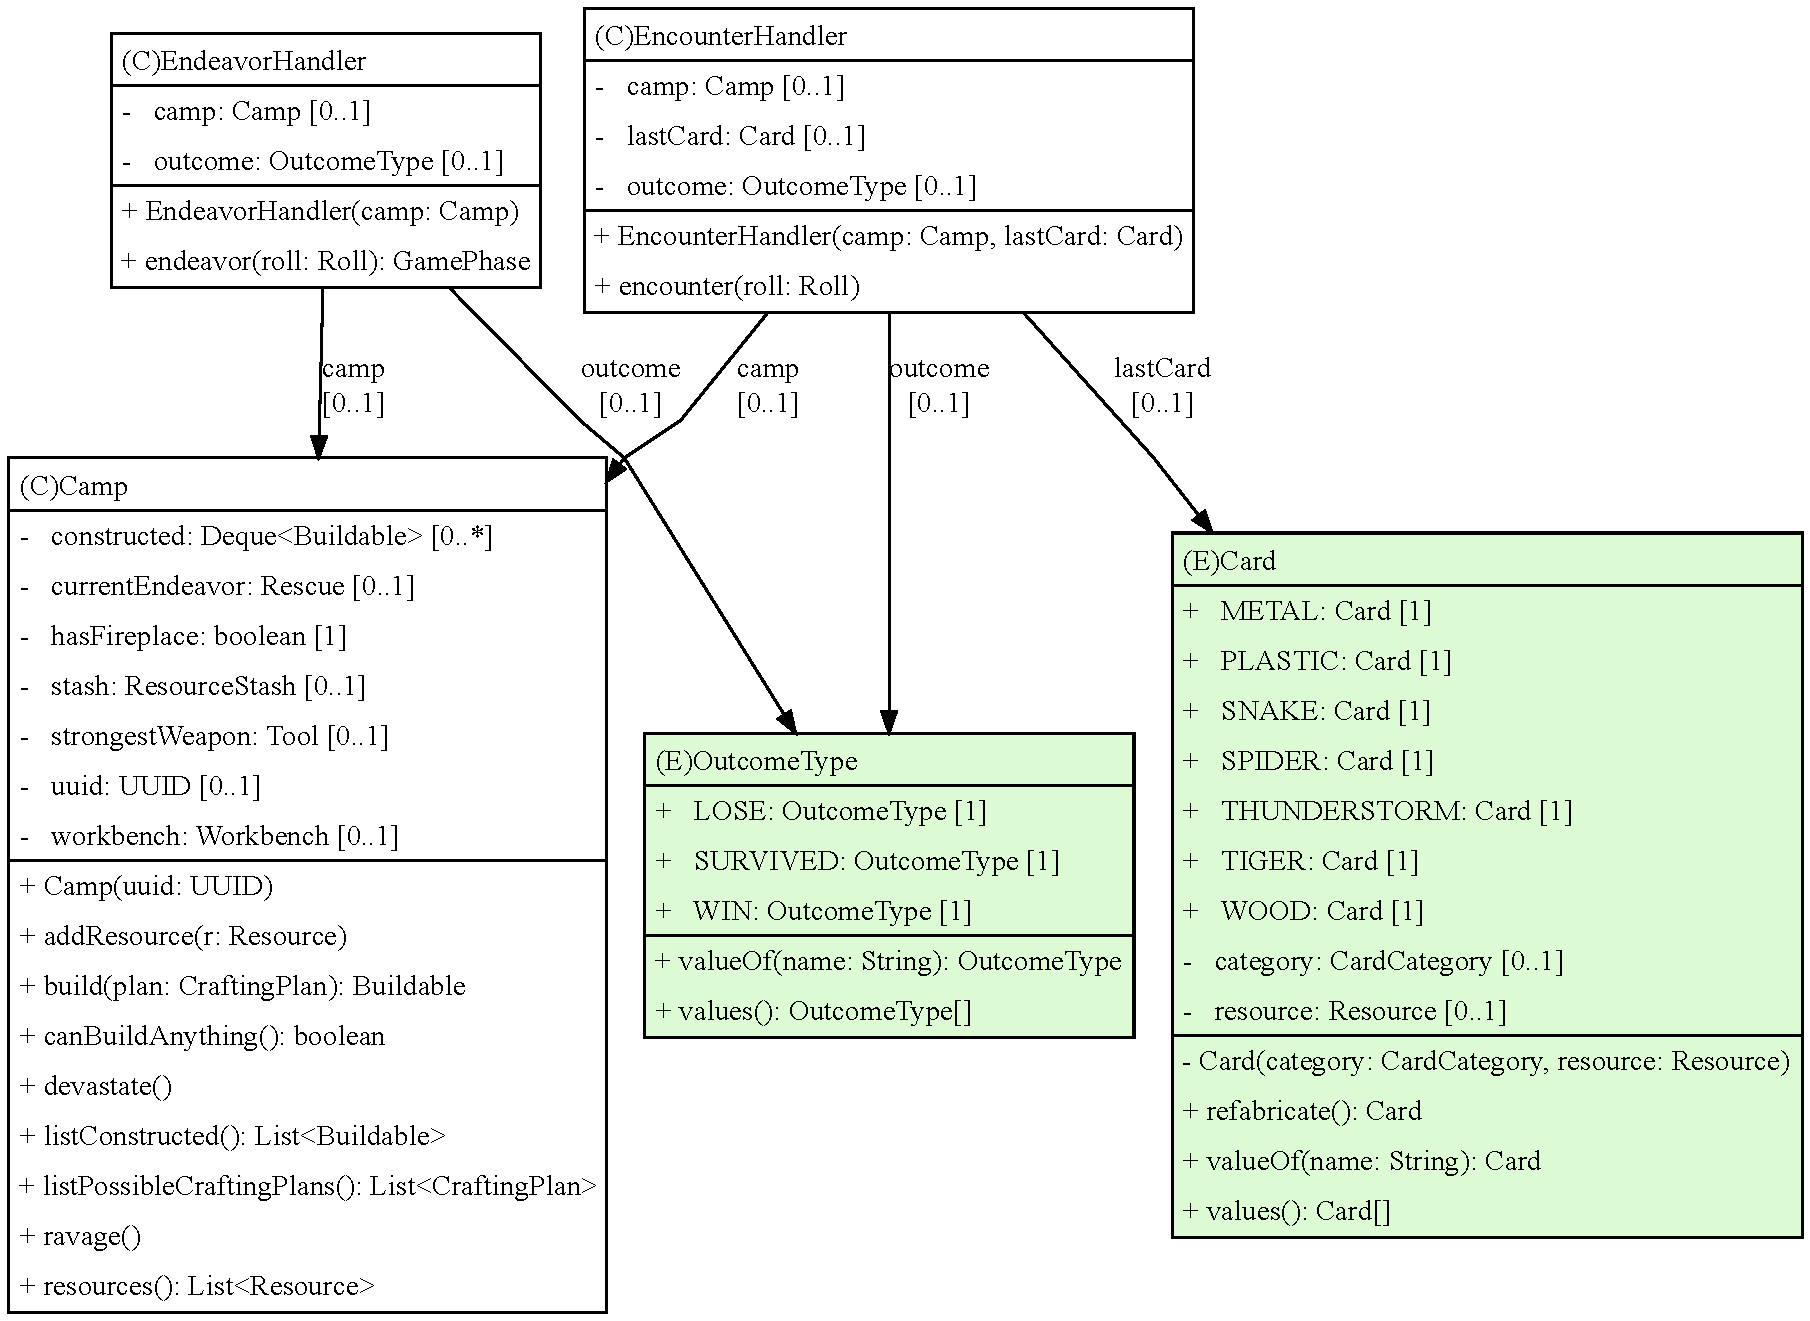
\includegraphics[width=1.\textwidth]{Bilder/RollHandler_fixed_structure.pdf} 
	\caption{\autoref{fig:srp-RollHandler} aufgeteilt in \textit{EndeavorHandler} und \textit{EncounterHandler}.}
	\label{fig:srp-RollHandler-fixed}
\end{figure} 


\section{Analyse Open-Closed-Principle (OCP)}

\subsubsection{Positiv-Beispiel:}

Das Positiv-Beispiel zum OCP wird konstituiert durch das \textit{Command}-Interface aus \texttt{ase.plugin.cli} 
und dessen Implementationen (z.B. \textit{RollDxCommand}) aus \texttt{ase.plugin.cli.commands} wie gezeigt in \autoref{fig:ocp-rolldx}. 
Die Main-Klasse kennt nur das Command-Interface und ruft darauf die \textit{execute}-Methode auf, 
die dann in den unterschiedlichen Command-Implementationen verschiedene Wirkungen auf das übergebene 
\textit{Game} haben. Dies ist auch die Begründung, wieso das OCP hier efüllt wird: Um einen neuen Befehl 
zu implementieren muss lediglich eine weitere Klasse hinzugefügt werden, die das Command-Interface implementiert.
Es muss dazu keine der bestehenden Command-Klassen angepasst oder geändert werden. 

Das OCP ist hier sehr sinnvoll, da für neue Features sehr wahrscheinlich regelmäßig neue Commands hinzugefügt 
werden müssen und dies soll somit möglichst einfach umsetzbar sein und keinen bestehenden Code breaken. 
Zuvor wurden die unterschiedlichen Befehle über zahlreiche \texttt{switch}-Blöcke realisiert 
(siehe z.B. Commit 034a5c28), was Änderungen des Programmcodes an vielen Stellen nötig machte, 
um einen neuen Befehl hinzuzufügen. Außerdem wurden Runtime-Exceptions geworfen, wenn vergessen wurde 
den Code an einer Stelle anzupassen. Durch das neue System müssen \textit{keine} \underline{Änderungen} 
(geschlossen für Änderungen) an vielen Stellen mehr durchgeführt werden, 
sondern nur noch \underline{Additions} durchgeführt werden (offen für Erweiterung).  

\begin{figure}[H]
	\centering
	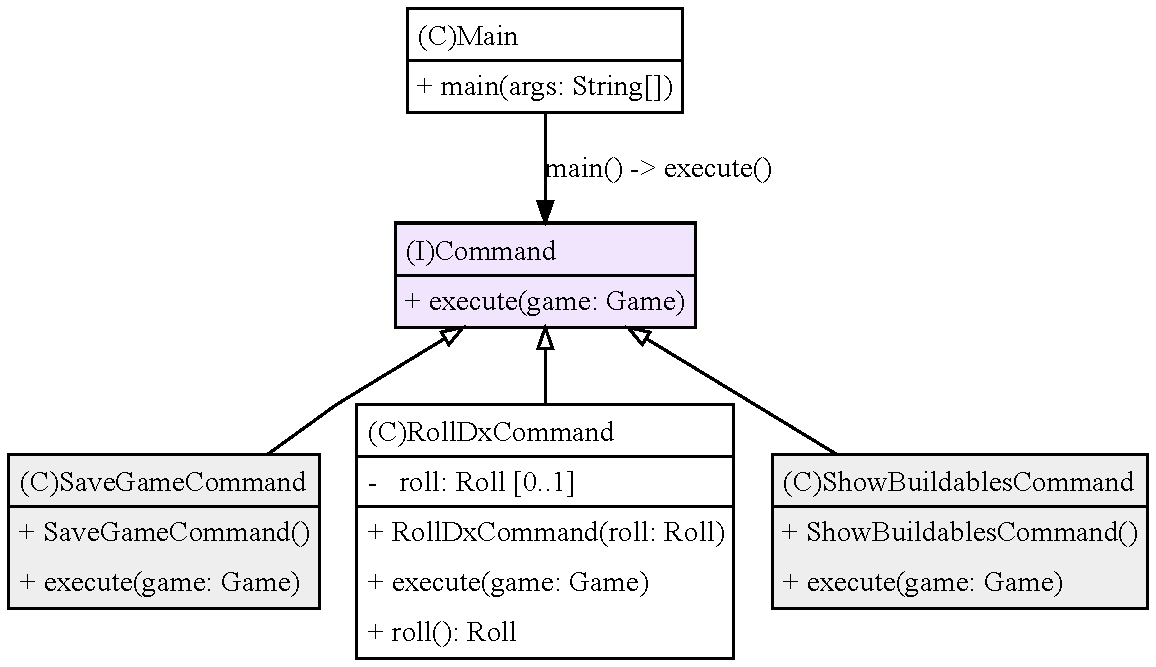
\includegraphics[width=0.7\textwidth]{Bilder/RollDxCommand_structure.pdf} 
	\caption{UML-Klassendiagramm vom \textit{RollDxCommand} und weiteren Commands, 
	wovon die meisten allerdings ausgelassen wurden der Übersichtlichkeit wegen.}
	\label{fig:ocp-rolldx}
\end{figure} 

\subsubsection{Negativ-Beispiel:}

\autoref{fig:ocp-CardInvalidator} zeigt das Negativ-Beispiel für das OCP. Die hier relevanten Klassen sind 
der \textit{CardInvalidator} und das \textit{Card}-Enum, welches eine \textit{CardCategory} und eine \textit{Resource} enthält. 
Der CardInvalidator zieht bisher eine Karte vom \textit{CardDeck} mit der \textit{draw}-Methode und invalidiert die Karte,
indem er deren Effekt einlöst. Dies wird mithilfe eines \texttt{switch}-Statements über die CardCategory der Karte entschieden.
Wenn nun also eine neue Karte mit einem neuen Karteneffekt hinzugefügt werden soll, muss also die \textit{draw}-Methode 
\underline{verändert} werden. Das OCP ist also nicht gewahrt. \\
\autoref{fig:ocp-CardInvalidator-fixed} zeigt eine mögliche Lösung, um das OCP einzuhalten: 
Das Card-Enum wurde mit einem Card-Interface mit der \textit{invalidate}-Methode ersetzt 
und die Karten (Metal, Wood, Tiger, etc.) sind nun Implementationen des Card-Interface und \textit{CardCategory} wurde entfernt.
Somit kann der CardInvalidator in 
\textit{draw} einfach die invalidate-Methode der gezogenen Karte aufrufen und die Karte führt selbst ihren Effekt aus. 
Somit können in Zukunft beliebig neue Karten eingeführt werden, für die einfach nur eine Implementation des Card-Interface 
geschrieben werden muss. Es ist keine Veränderung bestehenden Codes mehr nötig und somit wird das OCP mit dieser Lösung eingehalten.


\begin{figure}[H]
	\centering
	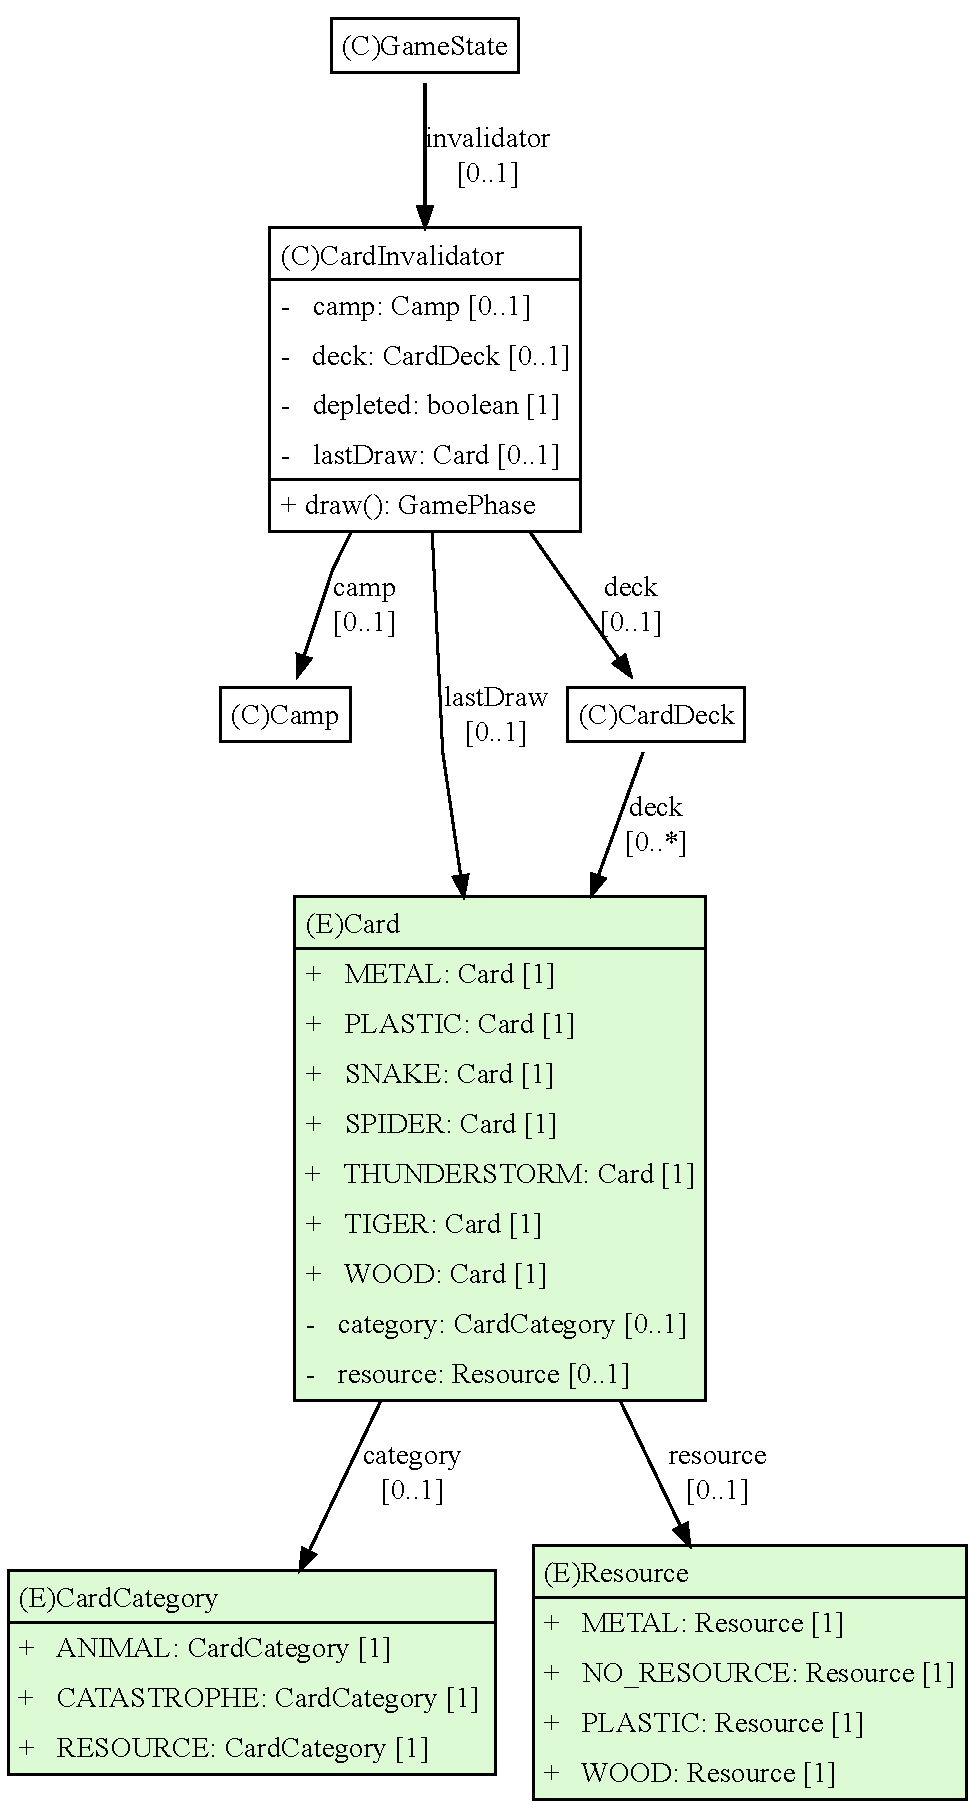
\includegraphics[width=0.5\textwidth]{Bilder/CardInvalidator_structure.pdf} 
	\caption{UML-Klassendiagramm von \textit{CardInvalidator} und \textit{Card}.}
	\label{fig:ocp-CardInvalidator}
\end{figure} 

\begin{figure}[H]
	\centering
	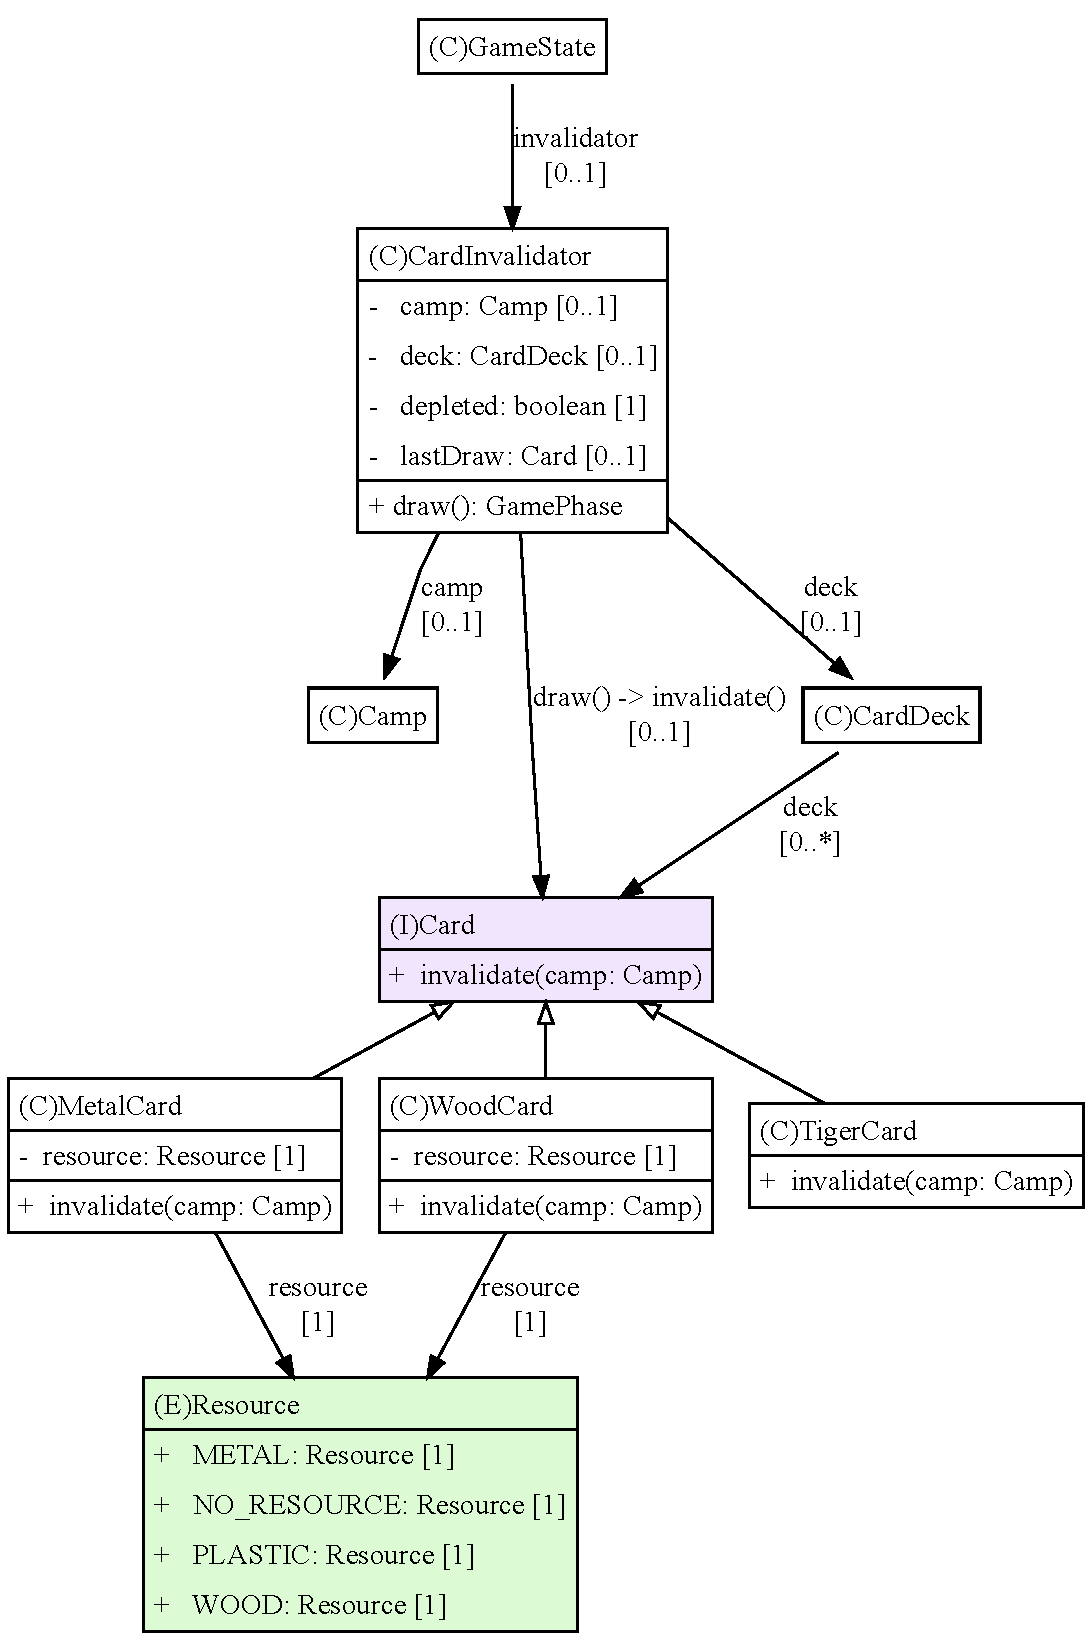
\includegraphics[width=0.55\textwidth]{Bilder/CardInvalidator_fixed_structure.pdf} 
	\caption{\autoref{fig:ocp-CardInvalidator} mit Card-Interface und Implementationen statt Card-Enum und CardCategory. 
	Aus Übersichtlichkeit wurden nicht alle Implementationen eingezeichnet.}
	\label{fig:ocp-CardInvalidator-fixed}
\end{figure} 


\section{Analyse Interface-Segreggation-Principle (ISP)}

\subsubsection{Positiv-Beispiel:} 

\autoref{fig:isp-Buildable} zeigt wie die Interfaces \textit{Buildable}, \textit{Tool}, \textit{Building} und \textit{Rescue} 
das ISP einhalten. Die Abhängigkeiten von anderen Klassen auf Tool, Building und Rescue sind aus Übersichtlichkeitsgründen ausgelassen.
Alle Interfaces enthalten nur eine Methode und alle Tool-, Building- und Rescue-Implementationen sind auch Buildables 
aber nicht anders herum. So können die Interfaces sehr flexibel angewandt werden und das ISP ist gewahrt. 

\begin{figure}[H]
	\centering
	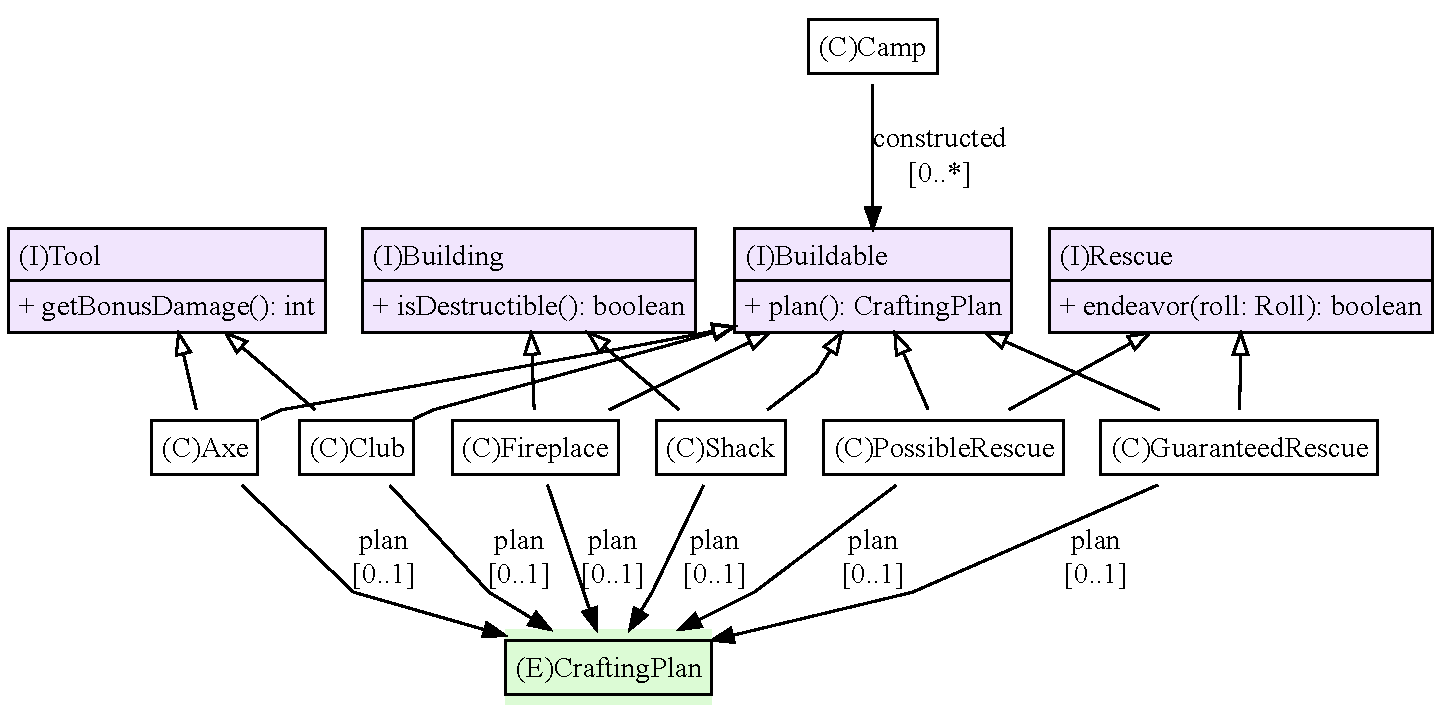
\includegraphics[width=0.9\textwidth]{Bilder/Buildable_structure.pdf} 
	\caption{UML-Diagramm von Buildable, Endeavor, Tool und Building und deren Implementationen.}
	\label{fig:isp-Buildable}
\end{figure} 

\subsubsection{Negativ-Beispiel:}

\begin{figure}[H]
	\centering
	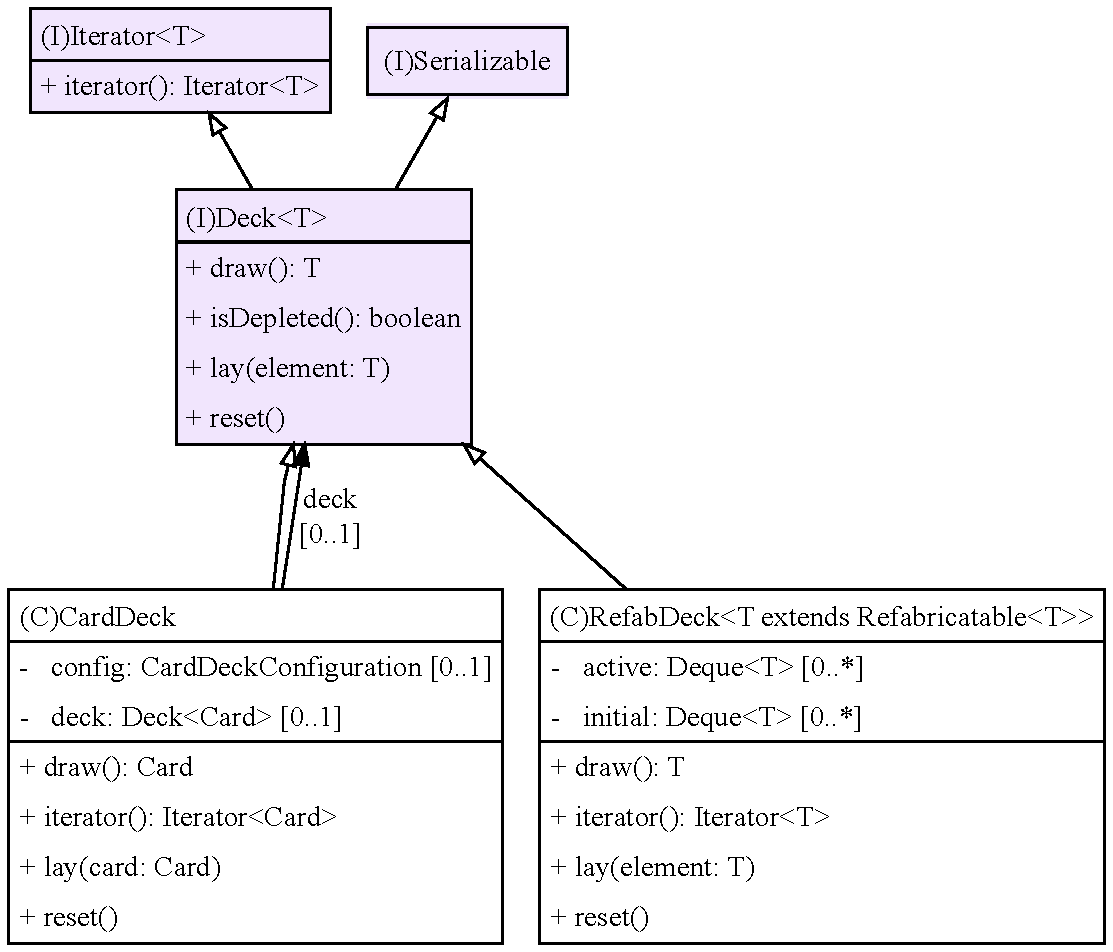
\includegraphics[width=0.5\textwidth]{Bilder/Deck_structure.pdf} 
	\caption{UML-Diagramm von \textit{Deck} und dessen Implementationen.}
	\label{fig:isp-Deck}
\end{figure} 


\autoref{fig:isp-Deck} zeigt das \textit{Deck}-Interface - das einzige Interface in der Applikation mit mehr als einer Methode.
Zunächst ist es allerdings diskutabel, ob es sich hierbei wirklich um ein Negativ-Beispiel handelt, da es sich bei dem Deck-Interface 
um eine Datenstruktur handelt, die besondere Eigenschaften aufweisen soll, wie z.B. dass der ursprüngliche Zustand der Datenstruktur 
bei Aufruf der \textit{reset}-Methode wieder hergestellt werden soll. Alle Methoden des Deck-Interfaces werden also 
gesammelt und gemeinsam benötigt, damit eine Klasse von der Abstraktion des Deck-Interfaces abhängen kann und den nötigen 
Funktionsumfang verwenden kann. Hier kann also erstmal das Deck-Interface nicht aufgeteilt werden. 
Außerdem hängt das Deck-Interface von dem \textit{Iterator}-Interface ab, sodass alle Implementationen von Deck auch 
automatisch Iterator implementieren müssen. Diese Funktion ist aber ebenfalls für ein Deck gewünscht - es soll möglich sein, 
mit einer Schleife über die Elemente des Deck zu iterieren. Damit ist also auch nicht das Iterator-Interface abspaltbar. \\
Allerdings wird es unmittelbar klar, dass das ISP hier eindeutig und ohne Diskussion gebrochen wird, wenn betrachtet wird, 
dass Deck ebenfalls das \textit{Serializable}-Interface beinhaltet, wodurch automatisch alle Implementationen das 
Serializable-Interface implementieren, was natürlich absolut \textit{keinen} Sinn ergibt. Es ist sogar gefährlich: 
Beim Implementieren des Deck-Interface wird dem Programmierer nicht klar, dass er die Implementation implizit und ohne Kenntnis als 
Serializable markiert, was ein großes Problem darstellen kann. \\ 
\autoref{fig:isp-Deck-fixed} zeigt nun, dass dieses Problem einfach behoben werden kann, indem die Implementationen explizit und direkt
Serializable implementieren und so bewusst die jeweilige Implementation als Serializable markieren. Damit ist das ISP wieder gewahrt,
da das Deck so weit wie sinnvoll möglich (Erläuterung s.o.) verkleinert wurde und die Implementationen nun von mehreren kleineren Interfaces abhängen,
anstelle von einem größeren abhängen. 

\begin{figure}[H]
	\centering
	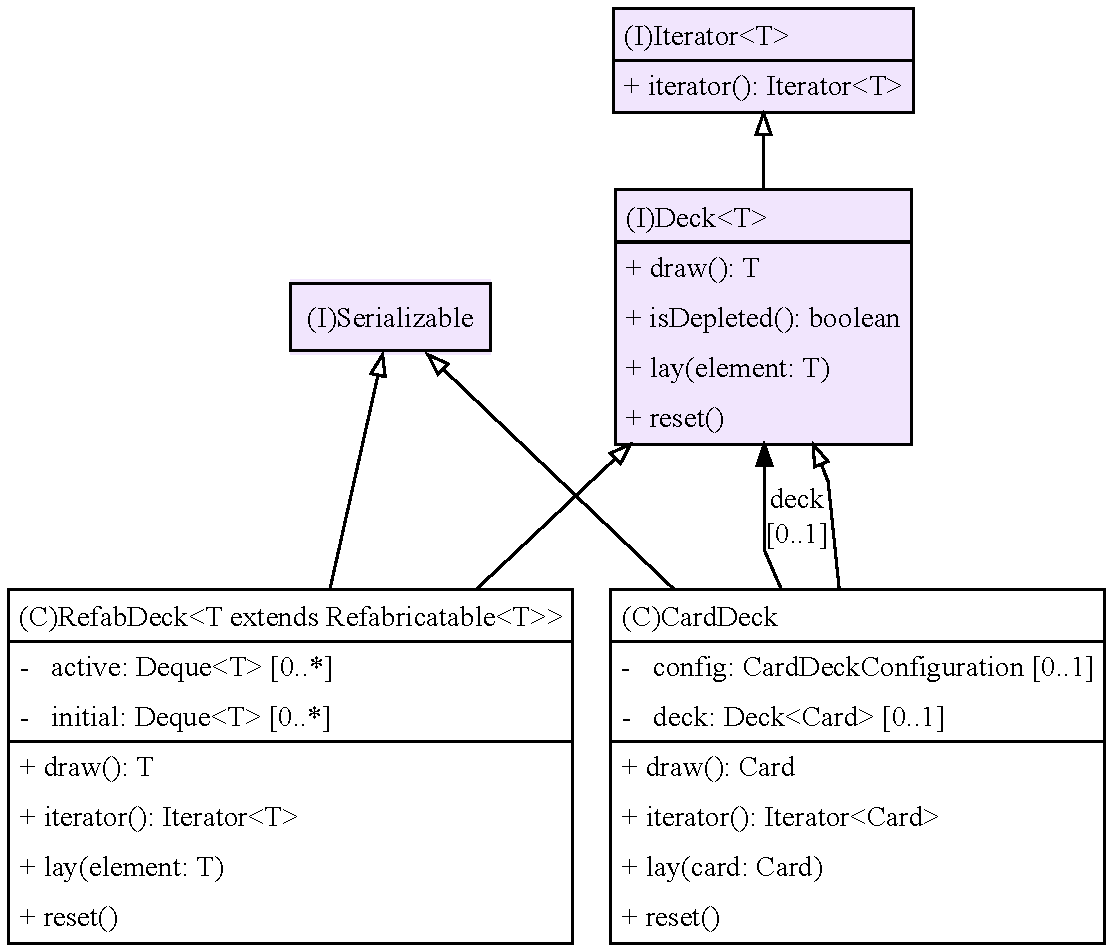
\includegraphics[width=0.5\textwidth]{Bilder/Deck_fixed_structure.pdf} 
	\caption{\autoref{fig:isp-Deck} mit abgespaltetem \textit{Serializable}-Interface.}
	\label{fig:isp-Deck-fixed}
\end{figure} 

